\documentclass[acronym, symbols]{fei}

\usepackage{subcaption}
\usepackage{chngcntr}
\usepackage{float}
\usepackage[portuguese]{algorithm2e}
\usepackage{biblatex}
\usepackage{amsmath}
%\usepackage[utf8]{inputenc}
\usepackage{chngcntr} %Faz com que o numero das notas de rodape aumente crescentemente
\usepackage{appendix}
\usepackage{amsfonts}
\counterwithout{footnote}{chapter}% "

% escrita que precede cada entrada na lista de ilustrações
\renewcommand{\cftfigurepresnum}{Figura }
\setlength{\cftfigurenumwidth}{5.7em}

\title{Fusão de sensores com Filtro de Kalman Estendido para controle de posição de robôs omnidirecionais}
\author{João Victor Lourenço Aguiar}
\cidade{São Bernardo do Campo}
\instituicao{Centro Universitário FEI}

\newacronym{kf}{KF}{Filtro de Kalman}
\newacronym{kg}{KG}{Ganho de Kalman}
\newacronym{ssl}{SSL}{\textit{Small Size League}}

\addbibresource{Referencias.bib}
%\bibliographystyle{plain}
\nocite{*}
\bibliography{Referencias.bib}
\graphicspath{ {Imagens/} }

\makeglossaries

\begin{document}
	
\maketitle

\begin{folhaderosto}
	Dissertação apresentada pelo Programa de Pós Graduação, Mestrado em Engenharia Elétrica do Centro Universitário FEI, como parte dos requisitos necessários para obtenção do título de Mestre em Engenharia Elétrica. Orientado pelo Prof. Dr. Flavio Tonidandel
\end{folhaderosto}
	
\begin{resumo}

	Este projeto propõe o desenvolvimento de um sistema de controle de posição para os robôs da categoria \textit{Small Size} da RoboCup de futebol de robôs, a fim de melhorar seu posicionamento ao realizarem jogadas e diminuir a dependência do sistema de câmeras disponibilizados pela liga durante os jogos da categoria. O sistema de controle utiliza um filtro de Kalman para realizar a fusão de sensores, que no caso serão os \textit{encoders} acoplados aos eixos dos motores utilizados para movimentação dos robôs, e uma IMU (\textit{Inertial Measurement Unit}, do inglês), composta por um giroscópio e um acelerômetro, disponível no hardware dos robôs.

\end{resumo}

\listoffigures
%\listoftables
%\listofalgorithms
\printglossaries
\tableofcontents

\chapter{Introdução}

	A categoria \textit{Small Size} de futebol de robôs da \textit{RoboCup} tem uma característica muito dinâmica por conta da velocidade da bola utilizada, que pode chegar a até 6,5 m/s devido a limitações impostas nas regras da categoria, fazendo com que os passes e chutes sejam muito rápidos \cite{rules}. Sabendo disso, para a realização das jogadas que o software propõe e ser capaz de acompanhar esse dinamismo, faz-se necessário que os robôs tenham um sistema de controle de posição confiável e efetivo.
	
	O sistema de controle atual é realizado a partir da imagem de câmeras posicionadas acima do campo. Elas detectam os padrões de cores posicionados em cima dos robôs e, assim, identificam sua posição em campo e o número do robô em questão. % É possível ver na Figura \ref{fig:color_patterns} os 16 números diferentes formados pelo padrão de cor que deve ser colocado em cima dos robôs para sua identificação pelo sistema de câmeras.
	
%	\begin{figure}[!htb]
%		\centering
%		\caption{Padrões de cores para identificação dos robôs.} 
%		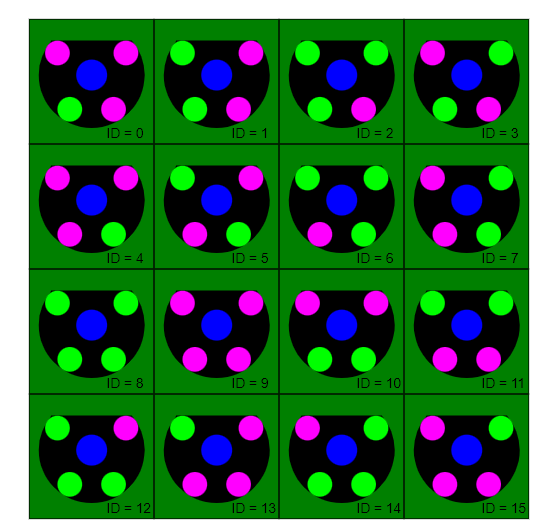
\includegraphics[width=0.5\textwidth]{Padrao_de_cores.eps}
%		\label{fig:color_patterns}
%		\smallcaption{Fonte: \textcite{rules}}
%	\end{figure}

	As câmeras captam as imagens, enviam-nas para um computador que faz a identificação dos robôs e as transmitem para os times pela rede as posições dos robôs e seus IDs. A partir disso, o software atual da equipe RoboFEI faz o controle de posição junto a estratégia. 
	
	Apesar do sistema de câmeras ser suficiente para o jogo, há diversos relatos de problemas com o controle de posição dos robôs por conta da latência consideravelmente alta da atualização do posicionamento deles. Segundo \textcite{tdpZJUNlict2020}, a câmera envia imagens a cada 15ms, mas por conta da filtragem realizada pelo sistema a atualização da imagem pode demorar de 3 a 4 ciclos (40 a 60ms), então há uma considerável demora para que o pacote atual com os dados seja recebido pelas equipes.
	
	O problema de alta latência de envio das imagens compromete a realização de jogadas durante as partidas e gera dificuldades no controle de posicionamento dos robôs. Isso faz com que a equipe fique estagnada e não tenha bons resultados em campeonatos internacionais, além de que a RoboFEI visa competir em uma divisão acima da que participa atualmente na \textit{RoboCup}, divisão essa que estão times mais desenvolvidos. Fica claro então a necessidade de tecnologias melhores para alcançar o nível das outras equipes da divisão.
	
	\section{Objetivos}
	
		Este estudo tem como objetivo desenvolver um novo sistema de controle de posição para os robôs da categoria \textit{Small Size} da equipe RoboFEI que não seja tão dependente do sistema de câmeras utilizado durante as partidas da categoria. Além disso, espera-se que o sistema possua uma latência de atualização menor e seja mais confiável e estável do que as câmeras em si. 
		
		Pretende-se utilizar um filtro de Kalman estendido a fim de unir dados de diferentes sensores, tais como giroscópio, acelerômetro, \textit{encoders}, e as próprias câmeras, que serão utilizadas para validação dos dados dos outros sensores.
		
		Após a implementação do novo sistema de controle de posição, espera-se que a equipe possa realizar as jogadas durante a partida com maior êxito, além de diminuir a quantidade de choque entre os robôs. Assim, espera-se bons resultados da equipe nos campeonatos da categoria \textit{Small Size} de futebol de robôs da RoboCup.
		
	\section{Justificativa}
	
		Como dito anteriormente, o sistema de câmeras utilizado nos jogos da categoria \textit{Small Size} de futebol de robôs da RoboCup não é suficiente para ter um controle adequado de posição dos robôs. Diferentes equipes já relataram dificuldades de controle de posição dos robôs por conta da alta latência de atualização das câmeras.
		
		Segundo \textcite{tdpZJUNlict2020}, há quatro grandes problemas com o sistema de visão global da categoria. Em primeiro lugar, como dito, é o problema de que a frequência de atualização de 75Hz não é o suficiente para um controle de movimentação rápido e acurado. Segundo, a informação das posições que é enviada para as equipes possui uma quantidade alta de ruído, o que compromete altamente o controle de orientação dos robôs. Terceiro, a informação enviada aos times é previamente processada, levando de 3 a 4 frames (40-60ms) entre coletar a informação original da visão até obter a informação da visão. Quarto, a taxa de quadros do sistema de visão é instável, o que pode gerar perda de frames e, consequentemente, torna a frequência do controle instável.
		
		A Figura \ref{fig:comparison_cameras_gyroscope} mostra uma comparação das informações de \textit{feedback} do ângulo de um robô. É possível notar um ruído muito alto da informação vinda da visão global, enquanto em relação ao giroscópio mal é possível notar algum ruido. Isso mostra o quão necessário é ter um sistema de controle que não seja totalmente dependente do sistema de câmeras da categoria.
		
		\begin{figure}[!htb]
			\centering
			\caption{Comparação da informação recebida pelo sistema de visão global e pelo giroscópio.} 
			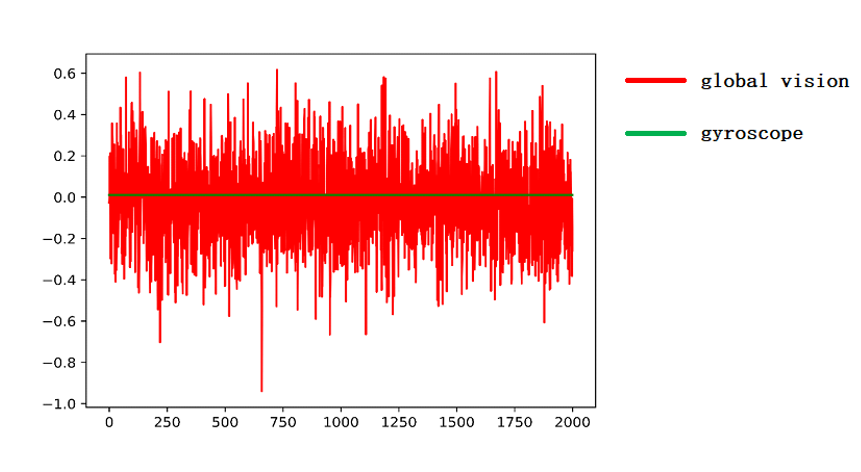
\includegraphics[width=0.8\textwidth]{Comparacao_cameras_giroscopio.png}
			\label{fig:comparison_cameras_gyroscope}
			\smallcaption{Fonte: Retirado de \textcite{tdpZJUNlict2020}}
		\end{figure}
	
		Além da equipe ZJUNlict em seu \textit{Team Description Paper} (TDP), que é o documento usado para se qualificar para a RoboCup e mostra toda inovação feita ao longo de um ano pelas equipes, a equipe RoboTeam Twente, em seu TDP de 2018, estima que o delay entre enviar um comando para o robô e notar uma resposta nas medições pode levar entre 80 e 150ms, dependendo da câmera sendo utilizada \cite{tdptwente2018}. Por conta disso, faz necessário um sistema que possua um delay relativamente menor para que o controle de posição dos robôs seja feito adequadamente. 
		
\chapter{Trabalhos relacionados}
	Nas seções a seguir serão descritos os trabalhos relacionados nas áreas de fusão de sensores, estimativa de posição de robôs móveis, filtro de Kalman 
		
\chapter{Revisão Bibliográfica}

	\section{\textit{RoboCup}}
	
		A ideia de robôs que jogam futebol foi proposta pela primeira vez pelo professor Alan Mackworth, em seu artigo \textit{On Seeing Robots} \cite{OnSeeingRobots}. Independentemente, em outubro de 1992, um grupo de pesquisadores japoneses organizou um workshop sobre os grandes desafios em IA, onde iniciaram-se as primeiras discussões sobre usar o futebol para promoção da ciência e tecnologia. Em junho de 1993 foi organizada uma competição de robótica e, em menos de um mês, pesquisadores de fora do Japão começaram a pedir que essa iniciativa fosse ampliada para um projeto conjunto internacional \cite{RoboCup}.
		
		A \textit{RoboCup} busca promover pesquisas na área de robótica e inteligência artificial com um objetivo final de vencer a seleção campeã do mundo em 2050 com uma equipe totalmente autônoma de robôs humanoides \cite{RoboCup}.
		
		O atual cenário competitivo da \textit{RoboCup} mostra equipes tanto do ensino superior quanto do ensino básico que disputam diversas categorias, em eventos tanto a nível nacional quanto a nível internacional, tais como \textit{RoboCup Soccer}, \textit{RoboCup Rescue}, \textit{RoboCup@home} e a \textit{RoboCup Junior}.
	
	\subsection{\textit{Small Size League}}
	
		A \textit{Small Size League}(SSL) uma das ligas mais antigas da \textit{RoboCup Soccer}, tendo o foco em solucionar o problema da cooperação e controle de robôs inteligentes num ambiente altamente dinâmico com um sistema híbrido centralizado/distribuído. A partida ocorre entre duas equipes utilizando seis ou onze robôs totalmente autônomos, que tem um máximo de diâmetro e altura, com algumas outras restrições \cite{RoboCup}. Além disso, os robôs da liga são omnidirecionais, o que proporciona jogos dinâmicos com jogadas imprevisíveis.
		
		Os jogos desta categoria são destacados por conta da alta velocidade tanto dos robôs, que podem chegar até 4m/s, quanto da bola utilizada, que pode chegar até 6.5m/s, mas também da quantidade de robôs numa partida, que acontece entre dois times que podem ter de 6 a 11 robôs num campo de 9m X 6m a 12m X 9m, dependendo da divisão da partida \cite{10332958}.
		
		Para realização da partida, um \textit{setup} específico é necessário. No caso, acima do campo são instaladas câmeras, as imagens delas são processadas por um computador central que disponibiliza, a partir de pacotes de rede, as posições $x$ e $y$ e a orientação $\theta$ dos robôs em campo, além das posições $x$ e $y$ da bola, como ilustrado na Figura \ref{fig:ilustracao_partida_ssl}.
		
		\begin{figure}[!htb]
			\centering
			\caption{Ilustração de uma partida da \acrshort{ssl}.} 
			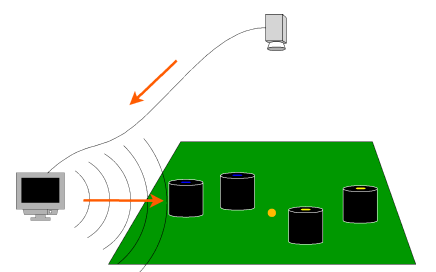
\includegraphics[width=0.5\textwidth]{funcionamento_ssl.png}
			\label{fig:ilustracao_partida_ssl}
			\smallcaption{Fonte: Retirado de \textcite{about-ssl}}
		\end{figure}
		
		Além disso, os robôs possuem limitações de tamanho, i.e., eles devem caber num diâmetro de 180mm e possuir uma altura máxima de 150mm \cite{rules}. A fim de lidar com essa limitação de dimensões e possuir robôs ágeis, as equipes utilizam um sistema de deslocamento omnidirecional, que é conseguido utilizando uma adaptação de rodas mecanum, em que os roletes são montados com uma certa angulação em relação ao eixo da roda \cite{aguiarreformulaccao}.
		
		
		
		
%	\section{Aquisição de dados}
%		A aquisição de dados é um passo importante para o desenvolvimento de qualquer sistema de controle de posição. Nessa etapa, basicamente, é feita a transformação dos dados crus dos sensores para valores com unidades que sejam utilizáveis para realização do controle.
		
	\section{Sensores}
	
		A utilização de sensores é parte essencial para o funcionamento correto de um robô. Segundo \textcite{de2017tipos}, o mais predominante em robôs industriais são robôs que são projetados para realizarem operações pré-programadas, que acabam não usufruindo de sensores para atingirem seu objetivo. Entretanto, para robôs mais complexos, os sensores acabam introduzindo um maior nível de inteligência para poder interagir com o meio que está inserido por meio de atuadores.
		
		Também de acordo com \textcite{de2017tipos}, a utilização de sistemas sensoriais faz com que robôs sejam mais facilmente adaptáveis a uma maior gama de tarefas, atingindo um maior grau de universalidade, diferente dos robôs pré-programados, que acabam realizando apenas uma única função. Um robô que, a partir da leitura dos sensores, possui sensações tal como um humano, é mais facilmente treinado para realização de tarefas complexas.
		
		\subsection{Tipos de sensores}
		
			De acordo com \textcite{sensorFusionKalmanFilter}, o sensores podem ser divididos em duas categorias principais: internos e externos. Essa diferenciação diz respeito a partir de onde vem a informação lida pelo sensor, ou seja, se é do mundo externo ou se é internamente do próprio robô.
			
			Sensores internos fornecem informações sobre parâmetros internos do robô, ou seja, medem variáveis físicas dele, como a velocidade e o sentido de rotação de um motor, ou o ângulo de uma junta, como exemplos. Alguns possíveis sensores que fazem parte desse tipo são: encoder, giroscópio, acelerômetro, bússolas.
			
			Já os sensores externos medem a relação entre o robô e o ambiente em que ele está inserido, que podem ser objetos naturais ou artificiais, como por exemplo a distância do robô até um objeto ou medidas químicas do ambiente. Alguns possíveis sensores que fazem parte desse tipo são: sensores de contato (bumpers), sensores de distância como laser, sonar e radar, entre outros.
			
			Ambos sensores possuem vantagens e desvantagens. Para períodos curtos de tempo, as medições de sensores internos são bem acuradas, embora a longo prazo as medidas normalmente passam a ter desvios e erros. Ao contrário disso, os sensores externos não tem problemas de desvio do sinal ao passar do tempo, mas as medidas deles normalmente não estão sempre disponíveis, ou seja, possuem um período grande para atualizarem suas medidas.
			
			Então, para obter resultados ótimos, ambos sensores são normalmente combinados, juntando as qualidades de ambos e fazendo com que as desvantagens deles sejam superadas. Por conta do erro de ambos os sensores, é realizada uma fusão das medidas dos dois tipos de sensores, o que irá produzir uma estimativa desejada da posição do robô.
			
			No caso deste projeto, os seguintes sensores serão utilizados e, então, explicados de maneira mais aprofundada: câmera, encoder, giroscópio e acelerômetro.
			
			\subsubsection{Sistema de câmeras}
			
				A câmera é um instrumento cujo uso em aplicações na área da robótica tem crescido bastante. Mapeamento, localização, navegação, desvio de obstáculos, reconhecimento de objetos e inspeção de qualidade são só alguns exemplos de possíveis utilizações de câmeras para realização de tarefas por parte de robôs. No centro dessa ascensão das câmeras está a evolução tanto dos processadores quanto dos algoritmos de visão computacional avançados.
				
				Segundo \textcite{cameras_technexion}, câmeras são cruciais no campo da robótica guiada por visão por aperfeiçoar as habilidades de percepção. Um robô pode aprender muito sobre seu arredor a partir dos dados visuais que câmeras coletam. Robôs podem obter informações valiosas desses dados utilizando diferentes métodos de processamento, permitindo então que o robô enxergue, compreenda e interaja com o ambiente de uma maneira mais profunda.
				
				No caso deste projeto, a utilização de câmeras se dá externamente aos robôs dentro da categoria SSL da RoboCup, já que, diferente da categoria \textit{Middle Size League}, o sistema de visão não é embarcada nos robôs, embora haja diversos estudos para alocar uma câmera dentro dos robôs da categoria de pequeno porte, como trazido por \textcite{melo2022embedded}.
				
				Detalhando um pouco mais o sistema de visão por câmeras da categoria SSL da RoboCup, atualmente utiliza-se uma ou duas câmeras, dependendo se o campo é da divisão A ou da divisão B. Independente do caso, a câmera fica posicionada acima do campo a 6 metros de altura e fica conectada a um computador central. Nele, a imagem é recebida, tratada e processada, identificando a posição da bola e dos robôs a partir do padrão de cor posicionado na parte de cima dos robôs, como é possível observar na Imagem \ref{fig:color_patterns} as 16 diferentes combinações possíveis \cite{10.1007/978-3-642-11876-0_37}.
				
				\begin{figure}[!htb]
					\centering
					\caption{Padrões de cores para identificação dos robôs.} 
					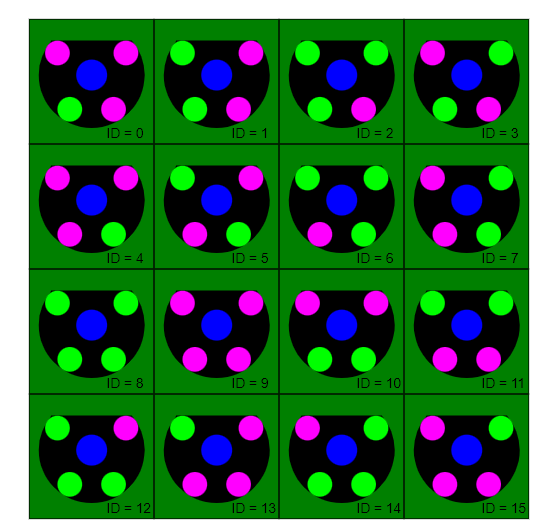
\includegraphics[width=0.5\textwidth]{Padrao_de_cores.eps}
					\label{fig:color_patterns}
					\smallcaption{Fonte: \textcite{rules}}
				\end{figure}
			
				Tanto o computador onde as imagens são processadas quanto o computador de cada uma das equipes estão conectadas numa mesma rede. Assim, após o processamento das imagens, a posição dos robôs e da bola são passadas para as equipes pela rede, por isso que o sistema de visão é dito compartilhado, pois ambas as equipes recebem as mesmas informações.
			
			\subsubsection{Encoder}
				
				Encoders são dispositivos utilizados a fim de medir o estado interno e a dinâmica de um robô móvel. Eles possuem uma vasta gama de aplicações fora da robótica e, por conta disso, robôs se aproveitaram dos benefícios da alta qualidade e baixo custo de sensores que oferecem uma excelente resolução de leitura. No mercado existem alguns diferentes tipos de encoders, como os ópticos e magnéticos. 
				
				No caso deste projeto, é utilizado um encoder do tipo óptico. Segundo \textcite{siegwart2011introduction}, este tipo de encoder se tornou o dispositivo mais popular para medição de velocidade e posição angulares de um motor, do eixo de uma roda ou mecanismo de direção.
				
				Um encoder óptico é basicamente um picador de luz mecânico que produz uma certa quantidade de pulsos na forma de um seno ou quadrado para cada revolução. No caso, o sensor consiste de uma fonte de iluminação, uma "grade" fixa que mascara a luz, um disco rotor com uma grade óptica fina que gira com o eixo e um detector óptico fixo. Ao passo que o rotor se movimenta, a quantidade de luz atingindo o detector óptico varia baseado no alinhamento das grades fixas e móveis. É possível observar a montagem e ter uma melhor ideia do funcionamento de um encoder óptico com a Figura \ref{fig:optical_encoder}.
				
				\begin{figure}[!htb]
					\centering
					\caption{Ilustração da montagem e funcionamento de um encoder óptico.} 
					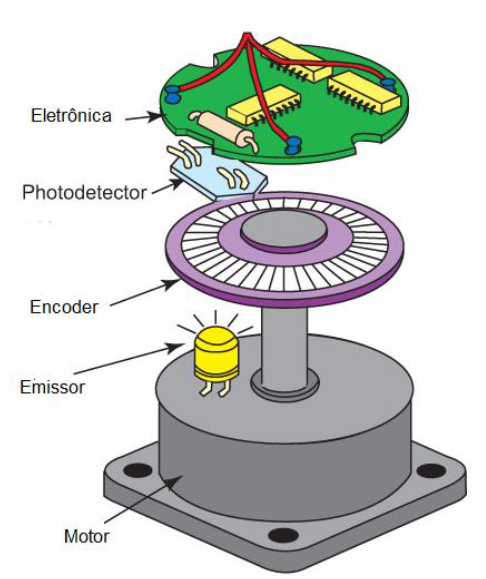
\includegraphics[width=0.5\textwidth]{encoder_optico.png}
					\label{fig:optical_encoder}
					\smallcaption{Fonte: Adaptado de \textcite{opticalencoder}}
				\end{figure}
			
			\subsubsection{Giroscópio}
			
				Giroscópios também são um dos principais sensores utilizados em robôs para realização de tarefas básicas como navegação. De acordo com \textcite{jeremydingman2020}, eles são componentes essenciais de sistemas complexos utilizados em todas aplicações aeroespaciais, industriais e na área da robótica. Giroscópios auxiliam desde aviões e barcos até drones e carros autônomos a navegarem.
				
				Segundo \textcite{s17102284}, giroscópios são dispositivos montados em uma estrutura e são capazes de realizar medidas de velocidade angular caso a estrutura esteja girando. Esse sensor pode ser utilizado de forma sozinha ou pode estar incluso em um sistema mais complexo, como uma bússola giroscópica, um IMU (\textit{Inertial Measurement System}, do inglês) ou um INS (\textit{Inertial Navigation System}, do inglês), por exemplo.
				
				No livro '\textit{Introduction to Autonomous Mobile Robot}', \textcite{siegwart2011introduction} trazem que giroscópios são sensores de direção que preservam sua orientação em relação a um \textit{frame} de referência fixo. Por isso, eles fornecem uma medida absoluta de orientação de um sistema móvel. 
				
				Também de acordo com \textcite{siegwart2011introduction}, os giroscópios são divididos em duas categorias: mecânicos e ópticos. Os primeiros dependem das propriedades de um rotor de rotação rápida, propriedade chamada de precessão giroscópica. Já os segundos são sensores de velocidade angular que utilizam dois feixes de luz monocromáticos, ou lasers, emitidos de uma mesma fonte
				
				No caso desse projeto, o giroscópio utilizado é o L3GD20, que é um sensor de velocidade angular de baixo consumo de energia capaz de realizar medidas nos 3 eixos \cite{datasheet_gyro}. Esse componente inclui o sensor e uma interface capaz de fornecer a medida de velocidade angular ao mundo externo por meio de uma interface digital (I$^2$C ou SPI).
			
			\subsubsection{Acelerômetro}
			
				O acelerômetro é mais um dos sensores que é utilizado para que o robô possua a habilidade de entender sozinho sua localização no espaço, o que é criticamente importante para alcançar com êxitos o objetivo determinado para o robô desenvolvido.
			
				Segundo \textcite{NISTLER2011413}, grande parte dos sistemas de odometria para aplicações em robótica possuem acelerômetros. Estes continuamente medem a aceleração do veículo, que é integrada para determinada a velocidade dele, e é integrado novamente para ter a medida da posição relativa ao ponto inicial.
				
				Entretanto, por conta da influência da gravidade, coriolis e componentes rotacionais de aceleração, sistemas de odometria baseados em acelerômetros estão sujeitos a diversos error dependendo do processamento das medidas do sensor. Também segundo \textcite{NISTLER2011413}, quando o robô se move numa superfície horizontal, a velocidade computada irá refletir a velocidade real do robô, mas em superfícies inclinadas, a velocidade medida irá incluir esses componentes, que não fazem parte da velocidade real.
			
				De acordo com \textcite{dadafshar2014accelerometer}, a operação básica de um acelerômetro recai na Segunda Lei de Newton, que diz que a aceleração de um corpo é diretamente proporcional, e na mesma direção, a força resultante atuante no corpo, e inversamente proporcional à massa do corpo, descrito na Equação \ref{eq:newton_second_law}.
				
				\begin{equation}\label{eq:newton_second_law}
					\overrightarrow{a}(m/s^2) = \frac{\overrightarrow{F}(N)}{m(kg)}
				\end{equation}
			
				Nota-se que a aceleração gera uma força que é capturada pelo mecanismo de detecção de força do acelerômetro. Então, o acelerômetro na verdade realiza medidas de força, e não aceleração, mas ele acaba medindo a aceleração indiretamente por meio da força aplicada em um de seus eixos.
				
				De acordo com \textcite{siegwart2011introduction}, os acelerômetros são separados dependendo do princípio físico utilizado para realizar a medição da deflexão da massa interna do sensor. Um mecanismo comum de detecção utilizado é a detecção por capacitância, que medem a deflexão ao medir a capacitância entre uma estrutura física e a massa interna. Outra alternativa de medição é a piezoelétrica, que é baseada na propriedade de certos cristais em gerarem tensão quando um estresse mecânico é aplicado neles, no caso a massa interna é posicionada no cristal e, então, quando uma força externa é aplicada a massa induz uma tensão que pode ser medida.
				
				No caso desse projeto, o acelerômetro utilizado é o LSM303DLHC, que é um sensor digital de aceleração linear capaz de realizar medidas nos 3 eixos, mas também é um sensor digital magnético nos 3 eixos também \cite{datasheet_accel}. O componente inclui uma interface serial $I^2C$ que suporta os modos padrão e rápido com 100kHz e 400kHz.
				
			\subsubsection{IMU (\textit{Inertial Measurement Unit})}
			
				A IMU(do inglês, \textit{Inertial Measurement Unit}), é um dispositivo que utiliza giroscópios e acelerômetros para estimar a posição, velocidade e aceleração relativos do veículo em movimento. Este componente se tornou comum em aviões e barcos, por exemplo, por estimar a posição do veículo em seis graus de liberdade, no caso: posição(x, y, z) e orientação (\textit{roll}, \textit{pitch}, \textit{yaw}) \cite{siegwart2011introduction}.
				
				Além disso, as IMUs comercializadas também estimam velocidade e aceleração. Considerando que a IMU possua 3 acelerômetros ortogonais e 3 giroscópios ortogonais, os dados do segundo são integrados para estimar a orientação do veículo enquanto os dados do primeiro são utilizados para estimar a aceleração instantânea do veículo.
				
				A aceleração é, então, transformada para o frame da navegação local por meio da estimativa atual da orientação do veículo relativo à gravidade. Então, o vetor gravidade pode ser subtraído das medidas, resultando numa aceleração que é integrada para obter a velocidade e, então, integrada novamente para obtenção da posição. Para sobrepor o problema da necessidade de conhecer a velocidade inicial, a integração é tipicamente iniciada no repouco, ou seja, velocidade igual a zero.
				
				IMUs são extremamente sensíveis na questão de erros de medidas tanto em relação ao giroscópio quanto ao acelerômetro. Por exemplo, o desvio no giroscópio inevitavelmente prejudica a estimativa da orientação do veículo relativa à gravidade, o que resulta numa cancelação incorreta do vetor da gravidade. Além disso, por exemplo, os dados do acelerômetro é integrada duplamente para obter a posição, então qualquer resíduo do vetor gravidade gera um erro que é duplamente integrado na posição. Por conta desse problema de desvio, é necessário alguma referência de alguma fonte externa de medida, como um GPS, câmera ou LIDAR.
				
	\section{Localização de robôs}
	
		Nessa seção serão comentadas as questões que envolvem como um todo a localização de robôs móveis. No caso, serão discutidos o problema geral da localização de robôs e seus principais problemas, suas diferentes instâncias e a questão da informação disponível para localização de robôs.
		
		\subsection{Introdução}
		
			A navegação é uma das competências mais desafiadoras necessárias em um projeto de robô móvel. De acordo com \textcite{siegwart2011introduction}, o sucesso da navegação depende do sucesso de 4 pilares principais: percepção, localização, cognição e controle de movimento. O primeiro é como o robô interpreta os dados dos sensores para extrair dados significativos. O segundo é a determinação da posição do robô no ambiente. O terceiro é sobre como o robô deve decidir como agir para atingir seus objetivos. O quarto define como o robô deve modelar as saídas dos seus motores para atingir a trajetória desejada.
			
			Este trabalho se debruça no pilar da localização basicamente. O problema da localização consiste em responder a pergunta "Onde estou?" do ponto de vista do robô, o que quer dizer que o robô precisa descobrir sua localização relativa ao ambiente em que ele se encontra. Quando fala-se sobre posição, quer dizer sobre as coordenadas $x$ e $y$ do robô, tal como sua orientação no sistema de coordenadas global.
			
			Como dito em \textcite{thrun2001robust}, o problema de localização de um robô é algo muito importante, sendo um componente chave em diversos sistemas robóticos autônomos de sucesso. Se um robô não sabe onde está relativamente ao ambiente, a tomada de decisão do que fazer é praticamente impossível, o robô precisa ter pelo menos uma certa noção de onde ele está para poder operar e agir de maneira certa. Segundo \textcite{borenstein1997mobile}, saber exatamente a posição de um robô é um problema fundamental em aplicações de robôs móveis para prover realmente capacidades autônomas.
			
			Problemas de localização são caracterizados pelo tipo de conhecimento que está disponível inicialmente e durante a execução. Basicamente, há três tipos de problemas de localização com diferentes graus de dificuldade, que são:
			
			\begin{itemize}
				\item \textbf{Rastreio de posição:} Assume que a posição inicial do robô é conhecida, então a localização do robô pode ser conseguida ao acomodar o ruído na movimentação do robô, geralmente o efeito desse ruído sendo pequeno. Esse problema é dito como local, já que a incerteza é local e restrita a uma região perto da posição verdadeira do robô, além de que a incerteza é geralmente aproximada por uma distribuição unimodal, como uma gaussiana.
				
				\item \textbf{Localização Global:} Aqui a posição inicial do robô é desconhecida, já que o robô é inicialmente colocado em algum local do ambiente, mas há a falta do conhecimento de onde é o local, ou seja, ele precisa se localizar do zero. As abordagens para localização global não podem assumir limite no erro da posição, assim como assumir distribuição probabilística unimodal é geralmente inapropriado.
				
				\item \textbf{Problema do sequestro de robô:} É uma variante do problema de localização global, mas nesse caso o robô sabe onde está localizado e de repente é "sequestrado" para outra localização sem que o robô esteja ciente disso. O problema é o robô detectar que foi sequestrado e, em seguida, descobrir sua nova localização. A importância prática disso, apesar de ser algo que não aconteça frequentemente, decorre que grande parte dos algoritmos de localização não garantem que nunca falharão.
			\end{itemize}
			
		\subsection{Os desafios da localização}
		
			Ao falar dos desafio da localização, \textcite{siegwart2011introduction} fala sobre a situação hipotética de utilizar um GPS (do inglês, \textit{Global Positioning System}) em um robô móvel e como o problema de localização estaria evitado, já que o sensor informaria a posição exata interna e externamente e, então, a questão "Onde estou?" sempre estaria respondida. Porém, infelizmente, esse sensor não é prático, já que o GPS atual tem uma acurácia de alguns metros, o que é inaceitável para localizar robôs móveis, além de não funcionar em ambientes internos. 
			
			Indo mais a fundo nas limitações do GPS, a localização é mais do que saber a posição absoluta do robô em relação à Terra, é também saber a sua localização relativa em respeito a, por exemplo, humanos, considerando a situação de um robô que tem que interagir com pessoas. Além do mais, se o robô planeja atingir uma localização específica, talvez seja necessário adquirir um modelo do ambiente (um mapa) e, então, identificar a posição relativa do robô nesse mapa. 
			
			Por conta da falta de acurácia e imperfeição de sensores e atuadores que a localização enfrenta desafios difíceis. Os principais aspectos que tornam o funcionamento de sensores e atuadores sub-ótimos são: ruído e \textit{aliasing} em sensores e ruído em atuadores.
			
			Sensores são a entrada fundamental do robô para o processo de percepção	e, portanto, o grau em que sensores podem discriminar o estado em relação ao mundo que o robô se encontrada é crítico. O ruído induz uma limitação na consistência das leituras de um sensor em um mesmo estado do ambiente. Geralmente, a fonte de problemas com ruídos em sensores é que algumas características não são capturadas pelo robô e, então, ignoradas. Resumindo, o ruído em sensores reduzem a informação útil da leitura deles, uma saída para isso é levar várias leituras em conta, aplicando fusão temporal ou fusão de diversos sensores para aumentar a qualidade geral da informação de entrada de robôs.
			
			Outra deficiência em relação aos sensores é a questão do \textit{aliasing}, que os leva a colherem pouco conteúdo informativo, o que acaba agravando o problema da percepção e, assim, dificultando a localização de robôs móveis. Um exemplo que mostra bem a questão do \textit{aliasing}, trazido em \textcite{siegwart2011introduction}, é que a utilização de um sonar em um robô móvel não traz a informação se algo que foi detectado é um humano que o robô deveria dizer "com licença" ou um objeto inanimado que o computador deveria recalcular o trajeto para ultrapassar. Ou seja, a quantidade de informações é geralmente insuficiente para identificar a posição do robô a partir de uma leitura de percepção única.
			
			Já o ruído em atuadores cai na questão de que uma única ação tomada por um robô móvel pode ter diferentes resultados possíveis, mesmo que da perspectiva do robô o estado inicial antes da ação tomada é bem conhecido. Em resumo, atuadores em robôs móveis introduzem incerteza sobre o estado futuro, como por exemplo, o ato de andar tende a aumentar a incerteza de um robô. A maior fonte de erro geralmente reside em um modelo incompleto do ambiente, como por exemplo o fato de o modelo não levar em conta que as rodas de um robô podem escorregar ou que um humano pode empurrar o robô, ou seja, não leva em conta possíveis fontes de erros que não podem ser modeladas, resultando numa falta de acurácia entre o movimento físico do robô, a movimentação pretendida pelo robô e a estimativa de movimentação pelo sensor.
		
		\subsection{Informação disponível}
			
			Para determinar sua localização, um robô tem acesso a dois tipos de informação, primeiro por meio de uma compreensão a priori obtida pelo próprio robô ou suprida por uma fonte externa numa fase chamada de "inicialização", segundo o robô obtém informação sobre o ambiente por meio de cada observação e ação realizadas durante a fase chamada "navegação". 
			
			Em geral, a informação a priori fornecida ao robô descreve o ambiente pelo qual o robô está navegando, ou seja, especifica algumas características que são variantes no tempo e assim podem ser utilizados para determinar a localização. Alguns exemplos desse tipo de informação podem ser mapas e relações causa-efeito.
			
			Robôs podem ter acesso a um mapa que descreve o ambiente em que está localizado. Os podem ser topológicos ou geométricos \cite{singhal1997issues}, o primeiro tipo descreve o ambiente em termos métricos, como por exemplo mapas de rodovias, já o segundo tipo descreve o ambiente em termos de características específicas em localizações e maneiras de ir de um local para outro. O mapa pode ser aprendido pelo robô previamente, ou fornecido por uma fonte externa, ou aprende enquanto navega pelo ambiente. Já as relações causa-efeito fornecem informações a priori ao robô por meio de uma dada entrada de observação, dizendo ao robô onde ele está a partir delas. 
			
			Já a informação de navegação é a que o robô reúne de seus sensores enquanto navega pelo ambiente. Um robô tipicamente performa dois tipos de ações ao navegar: ele anda ou age no ambiente por um lado, e sente o ambiente por outro lado.
			
			Um sistema de locomoção consiste de rodas, pernas ou trilhos, ou qualquer coisa que faça o veículo se movimentar pelo ambiente. A maneira na qual um sistema de deslocamento muda a localização contém informação de valor para estimar a localização, ou seja, saber os efeitos de ações executadas pelo sistema indica diretamente a localização do veículo depois da execução dessas ações.
			
			O robô sente o ambiente por meio de sensores, que indicam a informação de uma situação momentânea, chamada de observação ou medição, ou seja, essa informação descreve uma situação do ambiente do robô em um certo momento. Observações feitas do ambiente providenciam informação sobre a localização do robô que é independente de uma estimativa de localização anterior, dando ênfase que a informação dessas medições vem da observação do ambiente ao invés do próprio robô.
	
	\section{Fusão de sensores}
	
		\textcite{alatise2020review} trazem que robôs móveis autônomos estão se tornando mais proeminentes nos últimos tempos por conta do aumento de sua relevância e aplicações em diversas áreas, como em empresas, indústrias, hospitais, setor agrícola, realizando funções como carregamento de objetos pesados, monitoramento e busca. Por conta disso, a fusão de sensores vem sendo utilizada para solução de problemas como localização, mapeamento e navegação.
		
		A fusão de sensores é um tema que envolve uma grande multidisciplinaridade de áreas, por conta disso existem diversas definições do que é fusão de sensores na literatura, como a definição de \textcite{white1991data}, que coloca como um procedimento multi-nível que lida com a associação, correlação e integração de dados e informações de uma ou múltiplas fontes a fim de atingir posições distintas, determinar estimativas e completar avaliações oportunas de situações. Trazendo mais para o campo da robótica, \textcite{durrant1988sensor} traz a definição como sendo a combinação de dados de múltiplas fontes a fim de melhorar a performance de robôs móveis.
		
		Embora a utilização da fusão de sensores na robótica seja considerada relativamente nova, a ideia em si de unir sensores não é recente. Um exemplo muito bom para mostrar esse fato é que, de acordo com \textcite{hall1997introduction}, humanos e animais desenvolveram a capacidade de utilizar múltiplos sentidos para melhorar suas habilidades de sobrevivência, como no caso de um animal que não consegue ver ao redor de cantos ou por meio da vegetação, então o sentido de audição pode prover bons avisos de perigos. Assim, a fusão de sensores é naturalmente realizada por animais e humanos para uma melhor abordagem do ambiente ao redor e para identificação de ameaças.
		
		De acordo com \textcite{marton2013two}, a fusão de sensores é um método efetivo para solucionar o problema de localização precisa de robôs móveis. Nessa técnica, mais de um sensor é utilizado para obter a posição do robô e para uma combinação efetiva de diferentes medições a fim de gerar os estados estimados do sistema. Assim, a fusão de sensores permite a mitigação das limitações de diferentes sensores, obtendo uma posição mais precisa do robô.
		
		A seguir, serão comentadas as vantagens e desvantagens de utilizar fusão de sensores em sistemas inteligentes, além de apresentar três tipos de classificação dos diferentes métodos e técnicas de fundir dados de múltiplos sensores em um sistema.
		
		\subsection{Vantagens e Desvantagens}
		
			\textcite{elmenreich2002introduction} traz em seu trabalho algumas motivações para utilização da fusão de sensores e que, no caso, sistemas que empregam métodos de fusão contam com uma quantidade de benefícios em comparação a sistemas com um único sensor. O autor traz que a medida de um sensor físico geralmente sofre dos seguintes prolemas:
		
			\begin{itemize}
				\item \textbf{Privação de sensor:} a avaria de um sensor causa perdas de percepção no objeto desejado.
				
				\item \textbf{Limitado espaço de cobertura:} normalmente um sensor individual cobre apenas um região restrita.
				
				\item \textbf{Limitado tempo de cobertura:} alguns sensores precisam de um tempo de setup particular para performar e transmitir uma medida, assim limitando a frequência máxima de medições.
				
				\item \textbf{Imprecisão:} medições de um sensor individual são limitadas a precisão do elemento sensorial empregado.
				
				\item \textbf{Incerteza: } a incerteza depende mais do objeto sendo observado do que do instrumento de observação. A incerteza cresce quando características estão faltando, como uma oclusão, quando o sensor não pode medir todos atributos relevantes de percepção, ou quando a observação é ambígua. Um sensor sozinho não consegue reduzir a incerteza na sua percepção por conta da sua visão limitada do objeto.
			\end{itemize}
			
			Como comentado anteriormente, o principal propósito de sensores externos é prover ao sistema informação útil no que diz respeito a informações de interesse do ambiente. A fusão de dados de diferentes sensores traz diversas vantagens relacionadas a obtenção de informações mais precisas, que no caso são impossíveis de perceberem somente com os dados individuais. Segundo \textcite{luo1990tutorial}, os seguintes itens são as principais vantagens da fusão de dados de sensores.
			
			\begin{itemize}
				\item \textbf{Informação redundante:} a redundância num sistema é fornecida quando um grupo de sensores está fornecendo as mesmas características, mesmo que com uma diferente fidelidade, do ambiente. A fusão de informação redundante pode reduzir a incerteza geral e assim aumentar a acurácia com que os dados são percebidos pelo sistema, além de aumentar a confiabilidade no caso de erro ou falha em algum sensor.
				
				\item \textbf{Informação complementar:} a complementaridade de dados permite a observação de recursos que seriam impossíveis de serem percebidos utilizando somente a informação dos sensores operando separadamente. Por exemplo, caso os recursos a serem percebidos forem considerados dimensões em um espaço de recursos, então a informação complementar é fornecida quando cada sensor consegue apenas providenciar um subconjunto dos recursos que formam o espaço.
				
				\item \textbf{Informação mais oportuna:} A fusão de sensores permite com que a informação esteja disponível mais rapidamente em comparação com a velocidade que poderia ser fornecida por um único sensor, devido à velocidade real de operação de cada sensor, ou o paralelismo de processamento que é possível trazer como parte do processo de integração.
				
				\item \textbf{Informação menos custosa:} no contexto de um sistema com múltiplos sensores, a informação é obtida num custo menor quando comparada à informação equivalente que poderia ser obtida de um único sensor. A não ser que a informação desse único sensor seja utilizado em outra parte do sistema, então o custo total do sensor deve ser comparada com o custo total do sistema multisensor integrado.
			\end{itemize}
		
			Embora seja provado a qualidade da fusão de sensores, também de acordo com \textcite{luo1990tutorial}, existem alguns problemas associados com a criação de uma metodologia geral para fusão de diferentes sensores e eles se concentram em torno dos métodos utilizados para modelagem do erro ou incertezas no processo de integração dos dados, na informação sensorial e na operação do sistem em geral incluindo os sensores. Sendo assim, os seguintes itens são colocados pelo autor como potenciais problemas.
			
			\begin{itemize}
				\item \textbf{Erro na integração e fusão do processo:} o grande problema na integração de informação redundante de diferentes sensores é a determinação de que a informação de cada sensor está se referindo aos mesmos recursos do ambiente, embora esse problema seja mais presente no caso de correspondência e associação de dados em visão estéreo e em pesquisa de monitoramento de diferentes alvos.
				
				\item \textbf{Erro na informação sensorial:} é normalmente assumido que seja causado por um processo de ruído aleatório que pode ser adequadamente modelado como uma distribuição probabilística. O ruído é normalmente assumido como não sendo correlacionado no espaço ou tempo (também chamado de ruído branco), Gaussiano e independente. A maior razão para que essas informações sejam assumidas é que elas permitem a utilização de uma variedade de técnicas de fusão de sensores.
				
				\item \textbf{Erro na operação do sistema:}  quando o erro acontece durante a operação por conta do efeito de acoplamento entre componentes de um sistema, ainda é possível assumir que as medições de um sensor são independentes se o error, após calibração, é incorporado ao modelo do sistema por meio da adição de uma variável de estado extra. Em ambientes conhecidos a calibração de diversos sensores não será um problema complicado, mas quando os sistemas multisensores são utilizados em ambiente desconhecidos, pode não ser possível a calibração dos sensores.
			\end{itemize}
		
		\subsection{Classificação de técnicas}
			Após o entendimento do que é a fusão de sensores, como ela pode ajudar diferentes sistemas e alguns pontos dela que merecem certa atenção para evitar problemas, é necessário diferenciar as diversas técnicas que realizam essa função de unir dados de sensores. De acordo com \textcite{castanedo2013review}, esse tema é uma área multidisciplinar que envolve diferentes campos do conhecimento, então é difícil estabelecer uma classificação clara e estrita das diferentes técnicas. Por isso, foram escolhidas 2 maneiras para classificação dos diferentes métodos de fusão sensorial.
			
			\subsubsection{Classificação baseada na relação entre as fontes de dados}
				Essa classificação foi proposta por \textcite{durrant1988sensor}, que se baseou na relação entre as fontes e separou nas seguintes três categorias.
				
				\begin{itemize}
					\item \textbf{Complementar:} é o caso de quando os sensores não dependem diretamente entre si, mas podem ser combinados de uma maneira que entreguem uma visão mais completa do fenômeno sendo observado. Ou seja, a informação providenciada pelas diferentes fontes representam diferentes partes do cenário. Um exemplo que pode ser colocado são câmeras em uma sala sendo que cada uma acaba observando partes disjuntas.
					
					\item \textbf{Competitiva:} também chamada de redundante, é o caso em que cada sensor entrega medidas independentes de uma mesma propriedade e, assim, as informações podem ser utilizadas a fim de obter uma informação global mais confiável. \textcite{visser1999organisation} ainda separam essa categoria em dois - a fusão de dados de diferentes sensores ou a fusão de medições de um mesmo sensor tomadas em diferentes instantes. Um exemplo é o caso de dados vindo de áreas sobrepostas em redes de sensores visuais.
					
					\item \textbf{Cooperativa:} é quando as informações fornecidas por dois sensores independentes são utilizadas para conseguir alguma informação que não estaria disponível com os sensores funcionando sozinhos. De acordo com \textcite{brooks1998multi}, é a fusão mais difícil de projetar, já que o dado resultante está suscetível a problemas de todos os sensores sendo fundidos, o que geralmente diminui a acurácia e confiabilidade em relação às outras categorias. Um exemplo é uma fusão de dados multi-modal entre áudio e vídeo para gerar uma informação mais complexa.
				\end{itemize}
			
				A Figura \ref{fig:classificacao_fusao_de_sensores} representa claramente a diferença entre as três categorias de classificação proposta por \textcite{durrant1988sensor}.
			
				\begin{figure}[!htb]
					\centering
					\caption{Diagrama representando a diferença entre as fusões complementar, competitiva e cooperativa.} 
					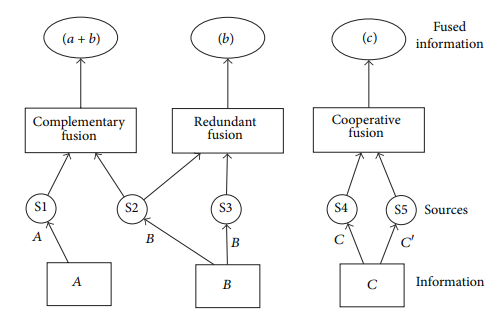
\includegraphics[width=0.8\textwidth]{classificacao_fusao_de_sensores.png}
					\label{fig:classificacao_fusao_de_sensores}
					\smallcaption{Fonte: Retirado de \textcite{castanedo2013review}}
				\end{figure}
			
			\subsubsection{Classificação em três níveis}
			
				A fusão de dados normalmente aborda três níveis de abstração: medidas, características e decisões. Essa maneira de classificar os diferentes métodos de fusão de sensores se baseia nessa ideia, dividindo-os em baixo, intermediário e alto nível, como é descrito a seguir.
			
				\begin{itemize}
					\item \textbf{Nível baixo:} também chamada de fusão de dados crus, essa categoria combina diferentes fontes de dados crus para produzir novos dados que espera-se que sejam mais informativos do que os de entrada.
					
					\item \textbf{Nível intermediário:} também chamada de fusão a nível de características, essa categoria combina diversos aspectos, como bordas, linhas, texturas ou posições em um mapa de características que pode então ser utilizado para segmentação ou detecção.
					
					\item \textbf{Nível alto:} também chamada de fusão de decisões, essa categoria combina decisões de diversos especialistas para obter uma decisão ainda mais precisa. Normalmente métodos bayesianos são empregados neste nível.
				\end{itemize}
			
			\subsubsection{Classificação baseada na entrada e saída do sistema}
			
				Esse sistema de classificação proposto por \textcite{dasarathy1997sensor} (por isso também chamado de modelo de Dasarathy) refinou o modelo de classificação em três níveis, dividindo as diferentes técnicas de fusão de sensores em 5 categorias baseado no nível de abstração dos dados de entrada e saída do sistema.
				
				\begin{itemize}
					\item \textbf{Entrada de dados-Saída de dados (DAI-DAO):} é o tipo mais básico de fusão de dados, nele há o processo de entradas e saídas de dados crus, os resultados são tipicamente mais confiáveis e acurados. Nesse caso a fusão é conduzida imediatamente depois da coleta de dados dos sensores.
					
					\item \textbf{Entrada de dados-Saída de características (DAI-FEO):} nesse nível o processo de fusão emprega dados crus das fontes para extrair características ou aspectos que descrevem a entidade do ambiente.
					
					\item \textbf{Entrada de características-Saída de características (FEI-FEO):} nesse nível tanto a saída quanto a entrada dos dados do processo de fusão são características. Assim, o processo aborda um conjunto de aspectos a fim de melhorar, refinar ou obter novas características.
					
					\item \textbf{Entrada de características-Saída de decisões (FEI-DEO):} este nível recebe um conjunto de características e, a partir delas, fornece um conjunto de decisões como saída do sistema. A maior parte dos sistemas que realizam uma decisão baseada no recebimento de dados de sensores entram nessa categoria.
					
					\item \textbf{Entrada de decisões-Saída de decisões (DEI-DEO):} esse tipo de classificação é também conhecida como fusão de decisão, já que funde decisões de entrada para obtenção de melhores ou novas decisões.
				\end{itemize}
				
				A Figura \ref{fig:classificacao_2_fusao_de_sensores} representa claramente a diferença entre as cinco categorias de classificação proposta por \textcite{dasarathy1997sensor}. Já a Figura \ref{fig:classificacao_3_fusao_de_sensores} relaciona e mostra as diferenças entre os modelos de classificação em três níveis e Dasarathy.
			
				\begin{figure}[!htb]
					\centering
					\caption{Diagrama representando a diferença entre as fusões baseadas no nível de abstração dos dados.} 
					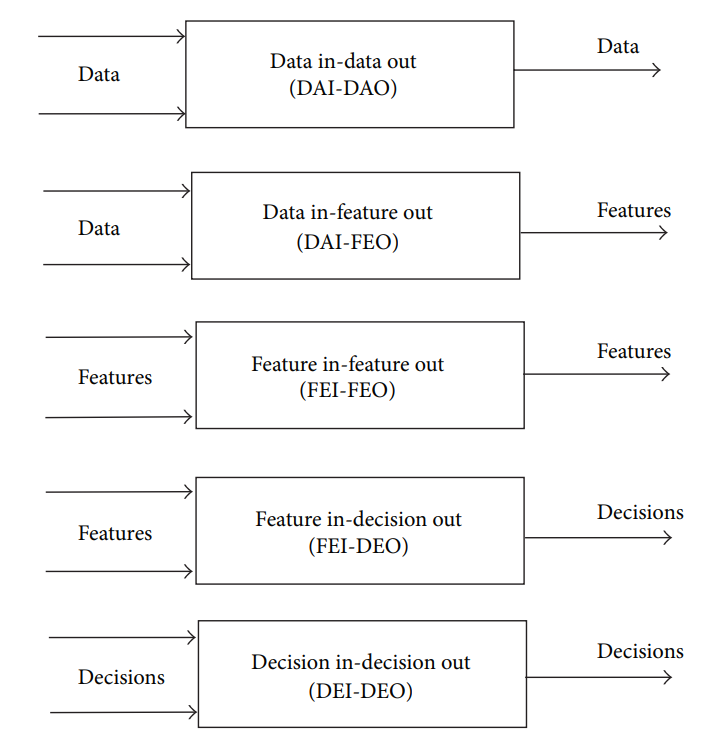
\includegraphics[width=0.6\textwidth]{classificacao_2_fusao_de_sensores.png}
					\label{fig:classificacao_2_fusao_de_sensores}
					\smallcaption{Fonte: Retirado de \textcite{castanedo2013review}}
				\end{figure}
			
				\begin{figure}[!htb]
					\centering
					\caption{Diagrama relacionando as classificações três níveis e Dasarathy.} 
					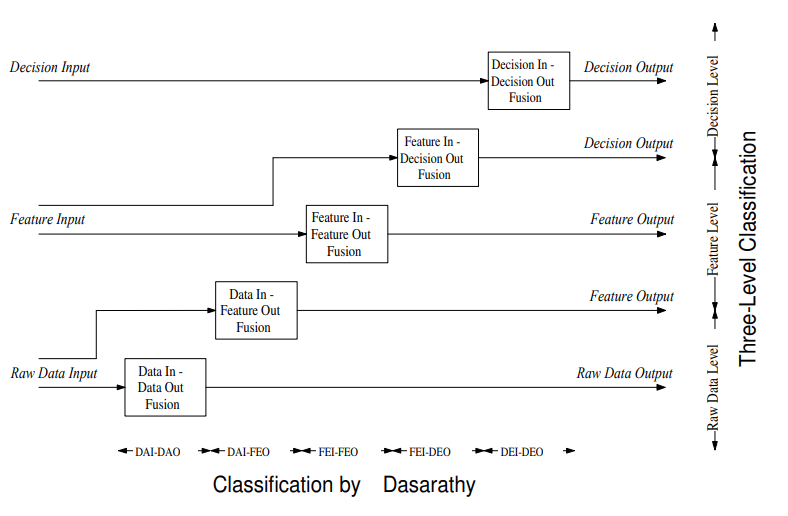
\includegraphics[width=0.8\textwidth]{classificacao_3_fusao_de_sensores.png}
					\label{fig:classificacao_3_fusao_de_sensores}
					\smallcaption{Fonte: Retirado de \textcite{elmenreich2002introduction}}
				\end{figure}
	
	\section{Filtro de Kalman}
		
		Nesta seção serão abordados os conceitos teóricos necessários para entendimento do tão divulgado e utilizado filtro de Kalman. Nela, serão apresentadas suas equações, as etapas do algoritmo.
		
		\subsection{Introdução}
		
			O filtro de Kalman foi inventado durante a década de 50 por Rudolph Emil Kalman como uma técnica para filtragem e predição em sistemas lineares. Desde então, por conta dos avanços na área de computação digital, o KF é objeto de extenso estudo e aplicações, particularmente na área de navegação autônoma ou assistida.
			
			O filtro de Kalman é um algoritmo que já foi utilizado em uma vasta gama de aplicações, principalmente na área de controle e na predição de sistemas dinâmicos \cite{phdthesisNegenborn}. Basicamente, existem dois tipos de aplicações para o KF, o primeiro caso é quando ele controla um sistema dinâmico (é utilizado para estimativa de estado, provendo uma informação que não pode ser medida diretamente por meio de um sensor, como em navios e aviões) e o segundo é quando o KF é utilizado para predição (ele prediz o futuro de sistemas dinâmicos que são difíceis de controlarem, como o fluxo de um rio durante uma enchente).
			
			Em suma, o filtro de Kalman é um conjunto de equações matemáticas que serve para estimar o estado de um sistema dinâmico linear com ruídos de tal maneira que a média do erro quadrático diminui de forma eficiente computacionalmente por ser um algoritmo recursivo. De acordo com \textcite{welch1995introduction}, o filtro é poderoso por conseguir estimar estados passados, presentes e futuros, até mesmo quando a natureza do sistema modelado é desconhecida.
			
			Quando fala-se sobre o estado de um sistema, coloca-se um vetor $x$ que consiste de $n$ variáveis que descrevem importantes propriedades de um sistema. Um exemplo de estado é a localização de um robô, que consiste das coordenadas $x$ e $y$ e a orientação $\theta$ de um robô.
			
			Como colocado anteriormente, robôs normalmente utilizam uma grande quantidade de sensores, cada um deles provendo a posição do robô, mas também cada um sendo sujeito a erros ou falhas no funcionamento. Então, a obtenção da localização ótima de um robô móvel deve levar em conta a informação gerada por todos sensores. Segundo \textcite{siegwart2011introduction}, o filtro de Kalman é uma técnica poderosa para atingir essa fusão de sensores por ser eficiente ao representar a função de densidade probabilística da crença do robô e até das leituras individuais dos sensores, resultando num algoritmo de processamento de dados recursivo ótimo.
			
			Entretanto, segundo \textcite{phdthesisNegenborn}, o fato de que as variáveis de um estado podem conter ruídos e não serem diretamente observáveis dificultam a estimação do estado. O KF possui acesso às medições do sistema para poder realizar a estimativa do estado, estas medições estão linearmente relacionadas ao estado e estão corrompidas por ruídos. Caso as fontes desses ruídos possuírem uma distribuição gaussiana, então a estimativa do KF é estatisticamente ótima para qualquer medida razoável de otimização.
			
			Também segundo \textcite{phdthesisNegenborn}, o KF processa todas medidas disponíveis de sensores para estimar o estado, tanto as medidas precisas quanto as imprecisas. Ele utiliza conhecimento do sistema e dinâmica dos sensores, descrição probabilística do próprio sistema e dos ruídos das medidas, e qualquer dado disponível sobre os valores iniciais do estado.
			
		\subsection{Premissas}
		
			A utilização do filtro de Kalman para predizer e corrigir a crença do estado presume a necessidade de um modelo tanto do sistema quanto medições. O \acrshort{kf} assume uma descrição de sistema dinâmico linear do sistema que está estimando o estado. O sistema dinâmico pode ser corrompido por fontes de ruídos, os quais o \acrshort{kf} assume que podem ser modelados por distribuições independentes, brancas, média zero e gaussianas.
			
			\subsubsection{Sistema dinâmico linear}
			
				Falando sobre o modelo do sistema, ele descreve como o verdadeiro estado do sistema evolui ao longo do tempo, utilizado pelo filtro para realizar predições sobre o estado. Basicamente, o \acrshort{kf} assume que o estado do sistema evolui de acordo com a Equação \eqref{eq:premissas_equacao_modelo_sistema}, onde o verdadeiro estado $x_k$ do sistema no tempo $k$ depende do estado um passo $x_{k-1}$ e algum ruído, a matriz $A$ tem tamanho $n \times n$ e relaciona os estados passo e atual, enquanto o vetor $w_k-1$ modela o ruído no sistema, modelando os efeitos de influências não modeladas no estado.
				
				\begin{equation}\label{eq:premissas_equacao_modelo_sistema}
					x_k = Ax_{k-1} + w_{k-1}
				\end{equation}
			
				O modelo de medição descreve como medições se relacionam com os estados. O filtro de Kalman necessita do modelo das medições a fim de corrigir a predição do estado quando uma medição está disponível. Basicamente, o \acrshort{kf} assume que as medições podem ser modeladas por um equação linear que relaciona o estado do sistema para uma medição, como a Equação \eqref{eq:premissas_equacao_medicoes}, em que $z_k$ depende linearmente do estado do sistema $x_k$, já a matriz H possui tamanho $m \times n$ e relaciona a medição com o estado, enquanto $v_k$ é o ruído nas medições.
				
				\begin{equation}\label{eq:premissas_equacao_medicoes}
					z_k = Hx_k + v_k
				\end{equation}
			
				Ambas Equações \eqref{eq:premissas_equacao_modelo_sistema} e \eqref{eq:premissas_equacao_medicoes} mostram que o estado $x_k$ no tempo $k$ não depende de todos os outros estados e medições dado $x_{k-1}$ e que a medição $z_k$ não depende de qualquer estado ou medida, o que torna o sistema um processo Markoviano.
			
			\subsubsection{Características do ruído}
				
				Uma característica necessária do ruído para o filtro de Kalman é a independência, que torna o cálculo envolvido na estimativa de estado mais fácil. De acordo com \textcite{phdthesisNegenborn} em geral é justo assumir que os ruídos no sistema e medição são independentes.
				
				Outra característica que simplifica a matemática envolvida no filtro de Kalman é o ruído branco, este tem poder em todas frequências do espectro e é completamente não correlacionado com ele mesmo em qualquer momento exceto o presente. Ou seja, os erros não se correlacionam pelo tempo, saber a quantidade de ruído neste momento não ajuda em predizer qual será a quantidade de ruído em outro momento.
				
				Uma terceira característica que é assumida é que o ruído possui média zero, o que implica que o erro no sistema e medição é aleatório. Um ruído aleatório significa que ele não é sistemático, ou seja, ele não possui um \textit{bias} constante, algumas horas ele é positivo, outras negativo, mas sempre média zero.
				
				A última característica importante que é assumida pelo filtro de Kalman é que o ruído é gaussiano, que é uma característica que lida com amplitude do ruído, colocando que a quantidade de ruído envolvida pode ser modelada por uma curva conforme a Figura \ref{fig:distribuicao_gaussiana}. Esta premissa é justificada ao assumir que os ruídos do sistema e medição são causados por diversas fontes pequenas de ruídos que, independente de suas distribuições, a soma delas será distribuída conforme uma gaussiana.
				
				\begin{figure}[!htb]
					\centering
					\caption{Exemplo de distribuição gaussiana.} 
					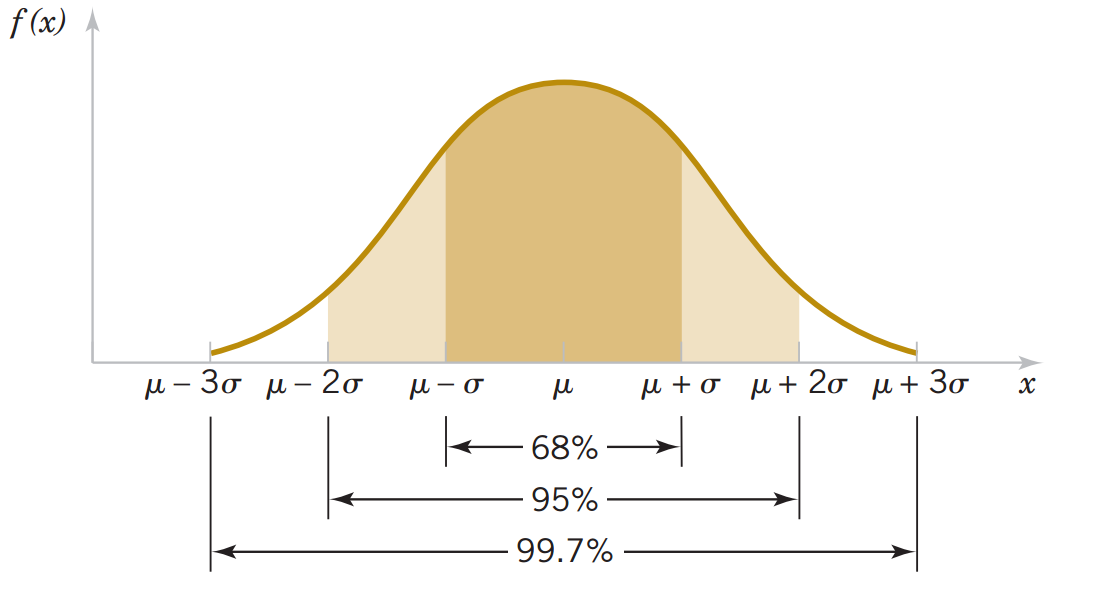
\includegraphics[width=0.6\textwidth]{distribuicao_gaussiana.png}
					\label{fig:distribuicao_gaussiana}
					\smallcaption{Fonte: Autor}
				\end{figure}
			
				Com as premissas da média zero e a distribuição gaussiana, os ruídos podem ser descritos de acordo com $N(\mu,\Sigma)$, que denota uma função gaussiana de média $\mu$ e covariância $\Sigma$.
		
		\subsection{Processo a ser estimado}
		
			O filtro de Kalman aborda o problema geral de tentar estimar o estado $x \in \mathbb{R}^n$ de um processo controlado em tempo discreto que é governado pela equação diferencial estocástica linear descrita pela Equação \eqref{eq:equacao_estado_sistema} com medição $z \in \mathbb{R}^m$, que é representada pela Equação \eqref{eq:equacao_medicao_sistema}. No caso, as variáveis aleatória $w_k$ e $v_k$ representam os ruídos do processo e das medições, respectivamente.
			
			\begin{equation} \label{eq:equacao_estado_sistema}
				x_k = Ax_{k-1} + Bu_{k-1} + w_{k-1}
			\end{equation}
		
			\begin{equation} \label{eq:equacao_medicao_sistema}
				z_k = Hx_k + v_k
			\end{equation}
		
			Assume-se que as variáveis $w_k$ e $v_k$ são independentes uma das outras, brancas, e com uma distribuição probabilística normal, segundo as probabilidades definidas na Equação \eqref{eq:equacao_probabilidade_variaveis_ruido}.
			
			\begin{equation} \label{eq:equacao_probabilidade_variaveis_ruido}
				\begin{split}
					p(w) &\sim N(0, Q) \\
					p(v) &\sim N(0, R)
				\end{split}
			\end{equation}
		
			Segundo \textcite{welch1995introduction}, a matriz de covariância do ruído do processo Q e a matriz de covariância do ruído das medições R podem variar a cada passo de tempo ou a cada medição, embora nesse caso será considerado constante.
			
			A matriz A da Equação \eqref{eq:equacao_estado_sistema} possui tamanho $n \times n$ e relaciona o estado no passo de tempo anterior $k - 1$ com o estado no passo de tempo atual $k$ na ausência de uma função ou ruído de processo. Já a matriz B possui tamanho $n \times l$ e relaciona a entrada de controle $u \in \mathbb{R}^l$ ao estado $x$. A matriz H possui tamanho $m \times n$ na Equação \eqref{eq:equacao_medicao_sistema} e relaciona o estado com a medição $z_k$.
			
		\subsection{Equações}
			
			De acordo com \textcite{welch1995introduction}, o filtro de Kalman estima um processo utilizando uma forma de controle por meio de feedback, nele o filtro estima o estado do processo em um dado instante e então obtém feedbacks na forma de medições, no caso ruidosas. Como tal, as equações do filtro de Kalman podem ser divididas em dois grupos: as equações de atualização de tempo e as equações de atualização medições. O primeiro grupo é responsável por projetar a frente no tempo as estimativas do estado atual e a covariância do erro para obter a estimativa a priori do próximo período de tempo. Já o segundo grupo é responsável pelo feedback, isto é, por incorporar uma nova medição na estimativa a priori a fim de obter uma melhor estimativa a posteriori.
			
			As equações de atualização no tempo podem ser chamadas como equações de predição, enquanto as equações de atualização de medição podem ser chamadas de equações de correção. Basicamente o algoritmo de estimativa final se assemelha com um algoritmo predição-correção para solução de problemas numéricos. A Figura \ref{fig:predicao_atualizacao_kalman} mostra o ciclo do filtro de Kalman, em que a predição projeta a estimativa do estado atual a frente no tempo, enquanto a correção ajusta a estimativa projetada por uma medição real naquele instante.
			
			\begin{figure}[!htb]
				\centering
				\caption{Ciclo do filtro de Kalman discreto.} 
				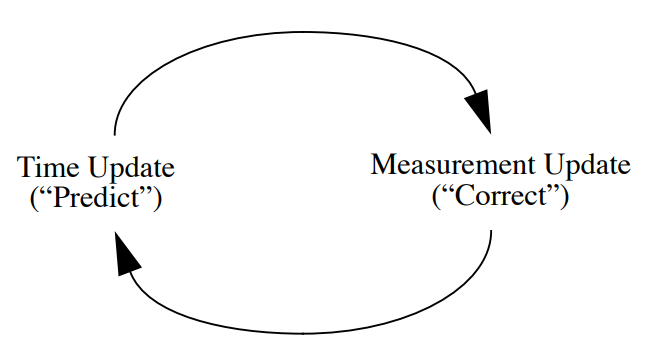
\includegraphics[width=0.6\textwidth]{predicao_atualizacao_kalman.png}
				\label{fig:predicao_atualizacao_kalman}
				\smallcaption{Fonte: Retirado de \textcite{welch1995introduction}}
			\end{figure}
			
			\subsubsection{Predição}
				A cada instante de tempo o sistema pode estar em um estado diferente. Portanto, o \acrshort{kf} calcula uma nova crença anterior a cada passo de tempo. As equações de predição (também chamada de atualização por tempo ou propagação) predizem o novo estado do sistema projetando à frente a crença mais recente, calculando a crença anterior $Bel^{-}(x_k) = N(\hat{x}_{k}^{-},P_{k}^{-})$, em que $\hat{x}_{k}^{-}$ e $P_{k}^{-}$ são definidos segundo a Equação \eqref{eq:equacao_predicao_kf}.
				
				\begin{equation} \label{eq:equacao_predicao_kf}
					\begin{split}
						&\hat{x}_{k}^{-} = A\hat{x}_{k-1}^{+} + Bu_{k-1} \\
						&P_{k}^{-} = AP_{k-1}^{+}A^{T} + Q_{k-1}					
					\end{split}
				\end{equation}
			
				O \acrshort{kf} calcula a estimativa de estado anterior $\hat{x}_{k}^{-}$ baseado tanto na última estimativa de estado posterior $\hat{x}_{k-1}^{+}$ quanto no modelo disponível do sistema. A melhor hipótese que o \acrshort{kf} pode fazer sobre o estado do sistema depois dele progredir um passo a frente no tempo é a melhor hipótese propagada pelo modelo que o \acrshort{kf} possui do sistema.
				
				Além disso, o filtro de Kalman também reconhece que a evolução do sistema está sujeita a ruídos e, assim, possui uma incerteza aumentada $P_{k}^{-}$ na estimativa do estado anterior. O primeiro termo da covariância do erro anterior $AP_{k-1}^{+}A^{T}$ propaga a incerteza da última estimativa posterior à frente para a estimativa atual do estado anterior. Já o segundo termo $Q_{k-1}$ é o ruído do sistema que corrompe o estado do sistema a cada passo de tempo.
			
			\subsubsection{Correção}
				As equações de correção(ou atualização da medição) lidam com as medições dos sensores. Elas são utilizadas apenas quando há a atualização da medição dos sensores. As medições providenciam informação direta sobre o estado atual do sistema. As equações de correção corrigem a crença mais recente ao incorporar a informação recebida das medições. As equações calculam a crença posterior $Bel^{+}(x_k) = N(\hat{x}_{k}^{+},P_{k}^{+})$, em que $\hat{x}_{k}^{+}$ e $P_{k}^{+}$ são definidos segundo a Equação \eqref{eq:equacao_medicao_kf}.
				
				\begin{equation} \label{eq:equacao_medicao_kf}
					\begin{split}
						&\hat{x}_{k}^{+} = \hat{x}_{k}^{-} + K_{k}(z_k - H\hat{x}_{k}^{-}) \\
						&P_{k}^{+} = (I - K_kH)P_{k}^{-} \\
						&K_k =  P_{k}^{-}H^T(HP_{k}^{-}H^T + R_k)^{-1}
					\end{split}
				\end{equation}
			
				A nova crença posterior é utilizada no próximo passo de tempo para calcular a nova crença anterior. A natureza recursiva do filtro de Kalman permite implementações práticas, já que nem todos os dados são necessários para estimar os estados.
				
				O filtro de Kalman calcula a estimativa do estado posterior combinando a estimativa do estado anterior com o ganho de Kalman $K_k$ vezes a diferença entre a medição $z_k$ e a previsão de medição $H\hat{x}_{k}^{-}$, chamada de inovação.
				
				O termo $H\hat{x}_{k}^{-}$ na Equação \eqref{eq:equacao_medicao_kf} é chamado de previsão de medição. Dadas que a estimativa do estado anterior ${x}_{k}^{-}$ e a matriz de medições $H$ do modelo de medição na Equação \eqref{eq:equacao_medicao_sistema}, o filtro de Kalman prediz qual medição irá receber. Assim, denota-se a previsão de medição segundo a Equação \eqref{eq:previsao_de_medicao_kf}.
				
				\begin{equation} \label{eq:previsao_de_medicao_kf}
					\hat{z}_k = H\hat{x}_{k}^{-} + \hat{v}_k
				\end{equation}
			
				No caso, o ruído de medição $\hat{v}_k$ é zero e a previsão de medição é uma variável aleatória que segue uma distribuição gaussiana, podendo notar isso ao analisar que ela depende linearmente da estimativa anterior do estado $\hat{x}_{k}^{-}$ e do ruído de medição, sendo que ambos são variáveis aleatórias gaussianas. Então, facilmente deriva-se que a predição de medida $\hat{z}_k$ segue a distribuição descrita na Equação \eqref{eq:distribuicao_predicao_medicao}.
				
				\begin{equation} \label{eq:distribuicao_predicao_medicao}
					\hat{z}_k = N_z( H\hat{x}_{k}^{-}, HP_{k}^{-}H^T + R_k)
				\end{equation}
			
				A diferença entre a medição $z_k$ e a medição prevista $x_{k}^{-}$ é chamada de inovação ou $\tilde{z}_k$ residual. A inovação diz quanto uma medida prevista difere de uma medição real, sendo definida segundo a Equação \eqref{eq:equacao_inovacao_medicao}. Caso a inovação seja igual a zero, então a medida prevista reflete exatamente a medição real, o que implica que o estado estimado com o qual a predição da medição foi realizada estava muito perto do verdadeiro estado que a medição foi feita. Entretanto, se existir uma diferença entre as medições prevista e observada, então a estimativa do estado anterior precisa ser atualizada com uma quantidade.
				
				\begin{equation} \label{eq:equacao_inovacao_medicao}
					\tilde{z}_k = z_k - \hat{z}_k
				\end{equation}
				
				A inovação depende das variáveis $z_k$ e $\tilde{z}_k$. Sabe-se que a medição real $z_k$ é dada que não adiciona nenhuma incerteza à inovação. A incerteza na inovação depende apenas da incerteza na predição de medida $\tilde{z}_k$ e é, assim, distribuído de forma gaussiana, como é demonstrado na Equação \eqref{eq:distribuicao_gaussiana_medicao}.
				
				\begin{equation} \label{eq:distribuicao_gaussiana_medicao}
					\begin{split}
						\tilde{z}_k \sim N_z(\mu_{\tilde{z},k}, \Sigma_{\tilde{z},k}) \\
						\mu_{\tilde{z},k} = z_k - \hat{z}_{k} \\
						\Sigma_{\tilde{z},k} = HP_{k}^{-}H^T +R_k
					\end{split}
				\end{equation}
			
				Nota-se que se há incerteza na medição real (por conta de incerteza na extração de uma característica, por exemplo), então a incerteza na inovação deve aumentar. A distribuição da inovação dá uma ideia de espalhamento das inovações, dando uma ideia dos erros nas estimativas de medições.
				
				O fator $K_k$ na Equação \eqref{eq:equacao_medicao_kf} é chamado de ganho de Kalman (\Gls{kg}, do inglês \textit{Kalman Gain}), que é o fator que fala até que ponto a inovação deve ser levada em conta na estimativa de estado posterior. Isso é determinado ao olhar a incerteza relativa entre a estimativa de estado anterior e a inovação da medição, como descrito na Equação \eqref{eq:equacao_medicao_kf}.
				
				A fim de comparar a incerteza da estimativa do estado anterior no espaço de estados com a incerteza da inovação no espaço de medição, o \acrshort{kf} converte a incerteza no espaço de medição para o espaço de estados por meio da matriz $H^T$.
				
				Quando a covariância do erro de medida $R_k$ se aproxima de zero, o \acrshort{kg} pesa mais para o lado da inovação, isto é, a inovação de medição $\tilde{z}_k$ é confiável para conter mais informações do que a estimativa do estado anterior, tal como descrito na Equação \eqref{eq:equacao_limite_ganho_kalman}. Ou seja, o \acrshort{kf} acredita menos no modelo do sistema e mais nas medições.
				
				\begin{equation} \label{eq:equacao_limite_ganho_kalman}
					\lim_{R_k \rightarrow 0 }K_k = H^{-1}
				\end{equation}
			
				Do contrário, quando a covariância do erro anterior $P^{-}_k$ se aproxima de zero, o \acrshort{kg} pesa menos para o lado do residual, isto é, quanto mais a covariância do erro anterior $P^{-}_k$ se aproxima de zero, menos a medição residual $\tilde{z}_k$ é levada em conta, como mostrado na Equação \eqref{eq:equacao_limite_ganho_kalman_2}. Ou seja, o \acrshort{kf} confia mais no modelo do sistema e menos nas medições.
				
				\begin{equation} \label{eq:equacao_limite_ganho_kalman_2}
					\lim_{P^{-}_k \rightarrow 0 }K_k = 0
				\end{equation}
			
				O filtro de Kalman também utiliza o ganho de Kalman para atualizar a incerteza que o próprio \acrshort{kf} possui na estimativa de estado posterior em ser o estado verdadeiro. Se o \acrshort{kg} está perto de $H^{-1}$ a inovação das medições é levada em conta quase completamente. Isso significa que o \acrshort{kf} confia que a inovação contém relativamente mais informação comparada com a estimativa de estado anterior. Isto resulta na diminuição máxima da incerteza do estado.
				
				Se as observações observam os valores de cada variável de estado diretamente e há uma grande quantidade de incerteza na estimativa de estado anterior relativa às medições, então o ganho de Kalman será perto de $H^{-1}$ e a estimativa do erro posterior estará próxima de zero. Isto vai levar ao \acrshort{kg} a não levar as próximas medições tanto em conta, já que a incerteza no estado é bem pequena, então o \acrshort{kg} também será. O tempo que leva até que o \acrshort{kf} leve novamente em consideração as inovações de forma significativa depende da quantidade de ruído do sistema adicionado na incerteza da estimativa de estado anterior a cada instante de tempo.
				
				Em resumo, o ciclo do filtro de Kalman pode ser entendido conforme ilustrado na Figura \ref{fig:ciclo_filtro_de_kalman_equacoes}, em que há o detalhamento das Equações de cada um dos passos do \acrshort{kf}, a predição e correção. Já a Figura \ref{fig:exemplo_filtro_de_kalman_covariancias} representa um exemplo em uma dimensão de como o filtro de Kalman realiza a predição e correção em termos de média e covariância.
				
				\begin{figure}[!htb]
					\centering
					\caption{Ciclo do filtro de Kalman discreto detalhado com as equações de cada passo.} 
					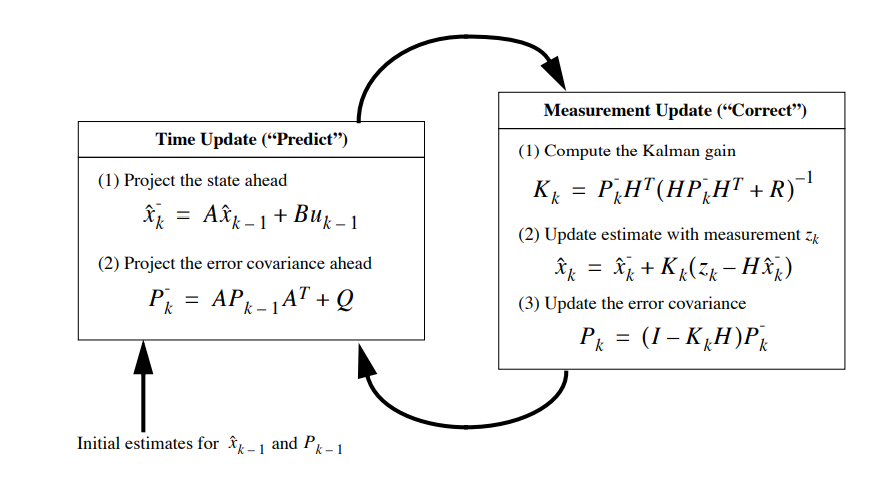
\includegraphics[width=0.8\textwidth]{ciclo_filtro_de_kalman_equacoes.png}
					\label{fig:ciclo_filtro_de_kalman_equacoes}
					\smallcaption{Fonte: Retirado de \textcite{welch1995introduction}}
				\end{figure}
			
				\begin{figure}[!htb]
					\centering
					\caption{Exemplo de predição e atualização das covariâncias do filtro de Kalman .}
					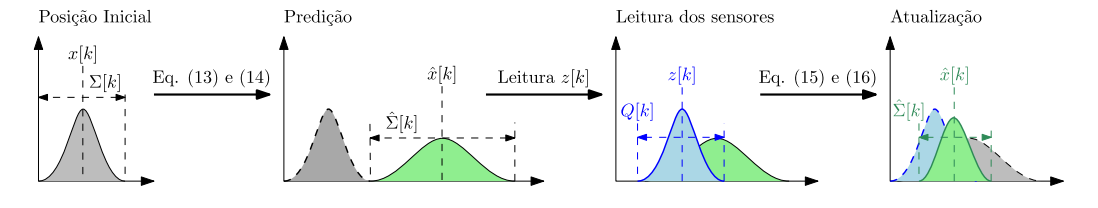
\includegraphics[width=0.9\textwidth]{exemplo_filtro_de_kalman.png}
					\label{fig:exemplo_filtro_de_kalman_covariancias}
					\smallcaption{Fonte: Retirado de \textcite{costaleonardo2023}}
				\end{figure}
		
		\section{Filtro de Kalman estendido}
			
\chapter{Metodologia}

	Neste capítulo serão apresentados o domínio de teste do projeto proposto, os testes a serem realizados, como os sensores serão combinados e quais métricas serão analisada para avaliação dos testes propostos.
	
	\section{Domínio de testes}
	
		Neste trabalho será utilizado o domínio de teste da categoria \textit{Small Size} de futebol de robôs da RoboCup \cite{RoboCup}. Nele, todas combinações de sensores serão testadas e comparadas. Para a realização dos testes propostos, será utilizado o campo do laboratório da equipe RoboFEI, que possui 4,3 X 3,6m, o que possibilita uma boa estimativa da movimentação do robô em um campo oficial da competição.
		
		O que torna a 
	
	\section{Combinação dos sensores}
	
		Nesta seção serão definidos os sensores a serem utilizados e como eles serão combinados para realizar a predição e correção do filtro de Kalman.
	
	\section{Testes}
	
		Nesta seção serão definidos os testes a serem realizados a fim de obtenção de dados relevantes para análise posterior das técnicas e combinações de sensores implementadas neste trabalho.
	
	\section{Avaliação}

		A fim de avaliar o sistema de controle de posição de robôs omnidirecionais proposto, que é baseado na fusão de diferentes sensores, além do sistema de visão global da categoria \textit{Small Size} para validação dos dados, utilizando um Filtro de Kalman Estendido, será realizada uma comparação com o sistema de controle de posição atual, que é totalmente dependente das câmeras utilizadas nas partidas. Também será feita uma análise do sistema de controle sem utilização do sistema de câmeras para validar a eficácia da fusão dos sensores, como se o robô estivesse se movimentando "às cegas".
		
		Os sensores que serão avaliados e, então, escolhidos posteriormente para serem utilizados no controle de posição, são: giroscópio e acelerômetro, que estão embutidos na IMU da placa de desenvolvimento STM32 utilizada no robô, odometria, que está relacionada com os encoders encaixados no eixo de cada um dos quatro motores utilizados para movimentação dos robôs, e também a câmera utilizada para visão global nas partidas da categoria \textit{Small Size} de futebol de robôs.
		
		A primeira avaliação a ser feita será a resposta do sinal de controle do sistema dado um entrada degrau para analisar a qualidade dos sistemas de controle em relação à orientação do robô. Basicamente, o robô estará com sua orientação em 0$^\circ$ e será enviado um sinal para que ele se posicione com sua orientação em 90$^\circ$, a resposta da orientação do robô será obtida e, então, forma-se o gráfico da orientação ao longo do tempo.
		
		A segunda avaliação a ser feita será a resposta do sistema de controle em relação a posição 2D do robô, isto é, nas coordenadas x e y. O teste consiste num trajeto, que no caso será um quadrado de lado 2 metros que o robô deverá seguir. O teste será realizado 20 vezes, e então serão analisados os erros médio em x e em y e o desvio padrão dos dados.
		
		O primeiro conjunto de controle a ser avaliado será a câmera junto da odometria, que é o sistema de controle atual utilizado pela equipe RoboFEI. O segundo conjunto de controle é o giroscópio, a câmera e a odometria. O terceiro conjunto é o acelerômetro, a câmera e a odometria, que servirá para avaliar as diferenças da utilização do acelerômetro e do giroscópio. O quarto conjunto será composto de todos sensores, isto é, giroscópio, acelerômetro, odometria e câmera. Já o quinto conjunto será feito tal como o quarto, mas sem a utilização da câmera, a fim de validar a qualidade da fusão de sensores sem a atualização do sistema de visão global.
		
		Ao fim dos experimentos, os dados serão avaliados e, então, o melhor sistema de controle de posição para os robôs da categoria \textit{Small Size} de futebol de robôs da RoboCup será escolhido avaliando os testes comentados acima. Assim, espera-se que a qualidade de jogo da equipe RoboFEI nas partidas aumente.
	
\chapter{Resultados Parciais}
	
	\printbibliography

\end{document}